% FIGURES

\begin{figure}[htb]
	\caption{\label{fig:1010} Forças internas atuando em um corpo em equilíbrio}
	\begin{center}
		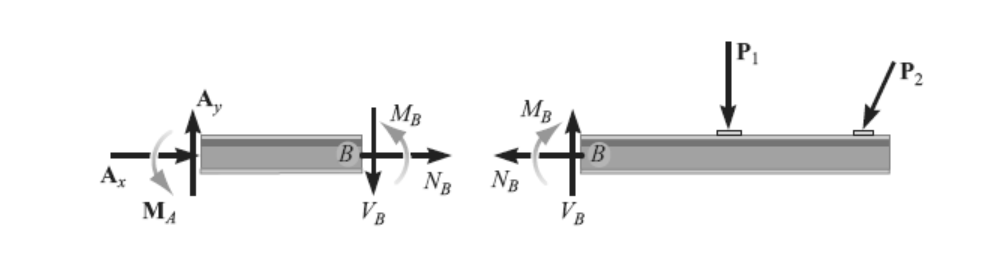
\includegraphics[width=\textwidth]{pictures/1010.png}
	\end{center}
	\fonte{\autocite{Hibbeler2010}}
\end{figure}


% EQUATIONS

\begin{equation}\label{eq:Eq_101}%
\mbox{\fontsize{17.28}{21.6}\selectfont\( %
\sum F_{x} = 0 \sum F_{y} = 0 \sum F_{z} = 0
\sum M_{x} = 0 \sum M_{y} = 0 \sum M_{z} = 0
\)} %
\end{equation}

\newline

sendo

$F_{x}$: Força de tração gerada pelos pneus

$\mu$: Coeficiente de atrito máximo do contato

W: Carga aplicada no eixo de tração


% DOUBLE EQUATIONS
\begin{equation}\label{eq:Eq_110}%
\mbox{\fontsize{17.28}{21.6}\selectfont\( %
\sum F_{x} = \sum F_{y} = \sum F_{z} = 0
\)} %
\end{equation}

\begin{equation}\label{eq:Eq_120}%
\mbox{\fontsize{17.28}{21.6}\selectfont\( %
\sum M_{x} = \sum M_{y} = \sum M_{z} = 0
\)} %
\end{equation}

Onde:

$F_{i}$: Forças axiais aplicadas no corpo no eixo "i"

$M_{i}$: Momentos aplicados no corpo no eixo "i"






